\begin{figure}[htbp]
\centering
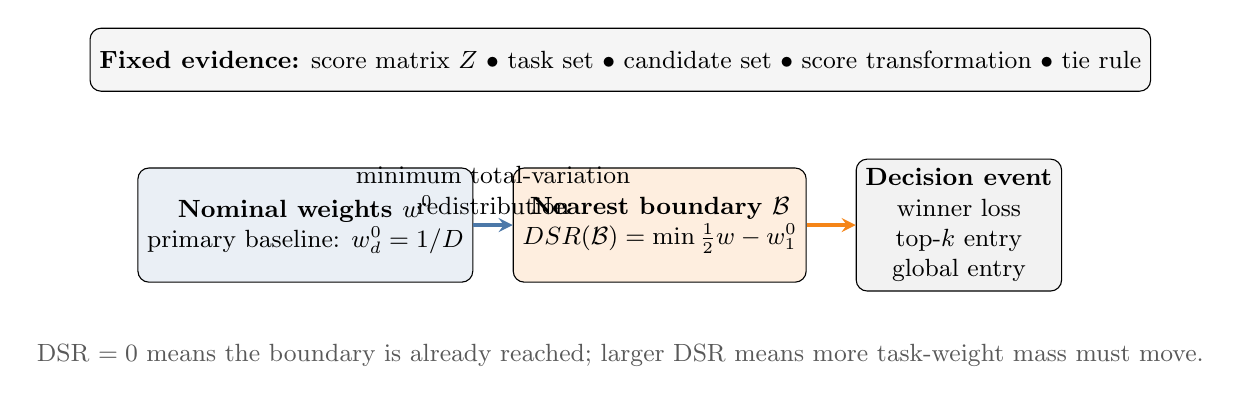
\begin{tikzpicture}[font=\small,>=stealth]
  \definecolor{pairblue}{RGB}{76,120,168}
  \definecolor{globalorange}{RGB}{245,133,24}
  \node[draw,rounded corners,fill=gray!8,minimum width=11.4cm,minimum height=0.8cm,align=center] (fixed) at (0,2.4)
  {\textbf{Fixed evidence:} score matrix $Z$ $\bullet$ task set $\bullet$ candidate set $\bullet$ score transformation $\bullet$ tie rule};
  \node[draw,rounded corners,fill=pairblue!12,minimum width=3.0cm,minimum height=1.45cm,align=center] (w0) at (-4.0,0.3)
  {\textbf{Nominal weights $w^0$}\\primary baseline: $w_d^0=1/D$};
  \node[draw,rounded corners,fill=globalorange!14,minimum width=3.5cm,minimum height=1.45cm,align=center] (b) at (0.5,0.3)
  {\textbf{Nearest boundary $\mathcal B$}\\$\operatorname{DSR}(\mathcal B)=\min \frac12\lVert w-w^0\rVert_1$};
  \node[draw,rounded corners,fill=gray!10,minimum width=2.6cm,minimum height=1.45cm,align=center] (event) at (4.3,0.3)
  {\textbf{Decision event}\\winner loss\\top-$k$ entry\\global entry};
  \draw[->,very thick,pairblue] (w0) -- node[above,align=center,text=black]{minimum total-variation\\redistribution} (b);
  \draw[->,very thick,globalorange] (b) -- (event);
  \node[align=center,text=gray!70!black] at (0,-1.35)
  {DSR $=0$ means the boundary is already reached; larger DSR means more task-weight mass must move.};
\end{tikzpicture}
\caption{Schematic of the DSR estimand. The score matrix and evidence state remain fixed; DSR is the minimum total-variation redistribution of task weight needed to reach a specified decision boundary. Schematic not to scale.}
\label{fig:dsr-concept}
\end{figure}

